%%================================================
%% Appendix I
%%================================================
\chapter[ภาพประกอบการสำรวจพื้นที่และการติดตั้งต้นแบบ]{\texorpdfstring{ภาคผนวก ฌ\\ภาพประกอบการสำรวจพื้นที่และการติดตั้งต้นแบบ}{Appendix I: Field Photos}}
\label{app:legacy_field_photos}

ภาคผนวกนี้แสดงภาพประกอบจากการสำรวจบริบทพื้นที่ การทดลองติดตั้งอุปกรณ์ และการรับฟังความคิดเห็นจากผู้ดูแล ภาพชุดนี้ใช้เป็นหลักฐานประกอบด้านสภาพแวดล้อมและการออกแบบต้นแบบ ไม่ได้ใช้เป็นหลักฐานว่าระบบผ่านการติดตั้งใช้งานจริงระยะยาวในสถานดูแลผู้สูงอายุ

\begin{figure}[!htbp]
    \centering
    \begin{subfigure}[t]{0.48\textwidth}
        \centering
        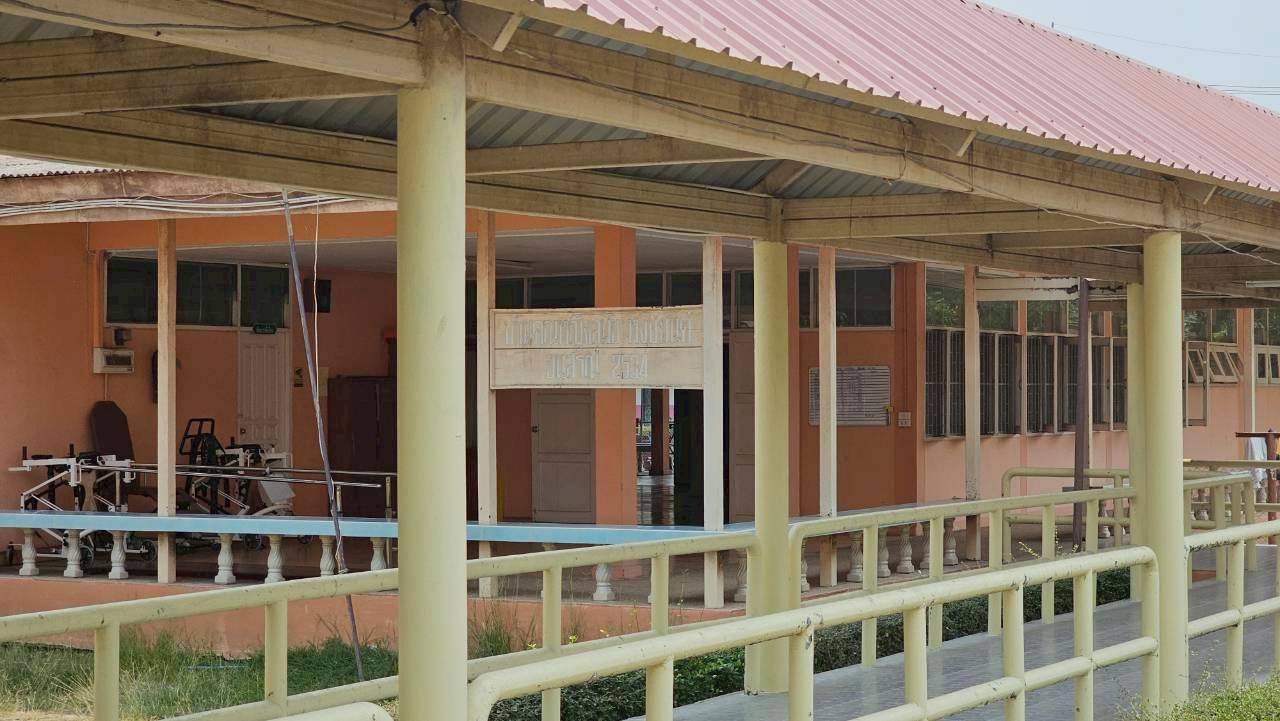
\includegraphics[width=\linewidth]{assets/appendices/legacy-field/facility-building.jpg}
        \caption{อาคารและพื้นที่บริการหลัก}
        \label{fig:appI_building}
    \end{subfigure}
    \hfill
    \begin{subfigure}[t]{0.48\textwidth}
        \centering
        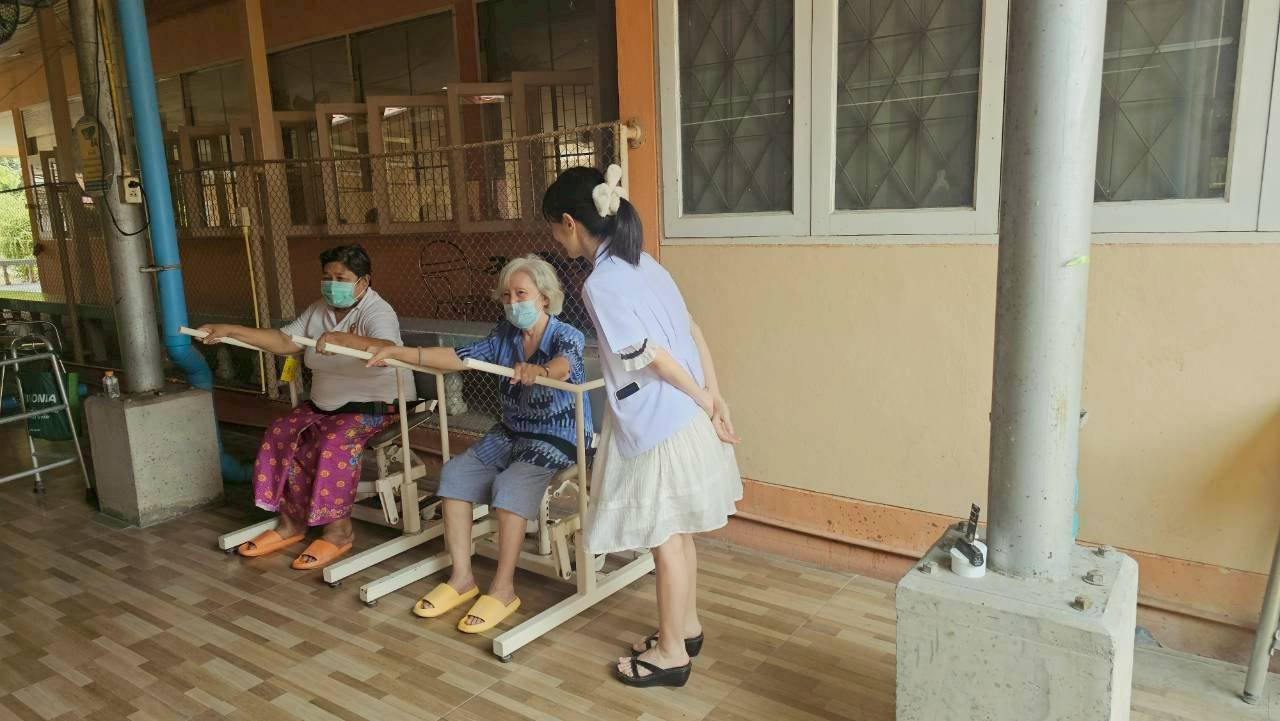
\includegraphics[width=\linewidth]{assets/appendices/legacy-field/node-install-1.jpg}
        \caption{การติดตั้ง node อ้างอิงสัญญาณ}
        \label{fig:appI_node_install1}
    \end{subfigure}
    \caption{บริบทพื้นที่และการติดตั้ง node อ้างอิงในสถานดูแล}
\end{figure}

\begin{figure}[!htbp]
    \centering
    \begin{subfigure}[t]{0.48\textwidth}
        \centering
        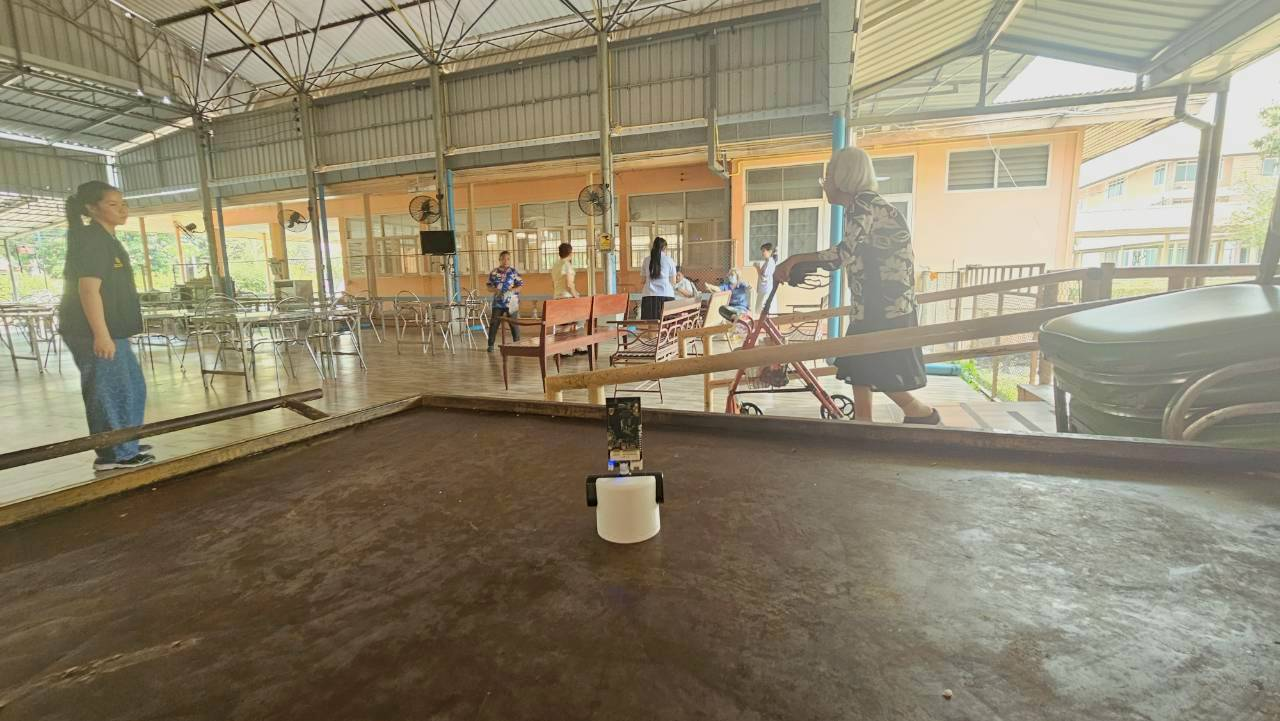
\includegraphics[width=\linewidth]{assets/appendices/legacy-field/node-install-2.jpg}
        \caption{ตำแหน่งติดตั้ง node อีกมุมมองหนึ่ง}
        \label{fig:appI_node_install2}
    \end{subfigure}
    \hfill
    \begin{subfigure}[t]{0.48\textwidth}
        \centering
        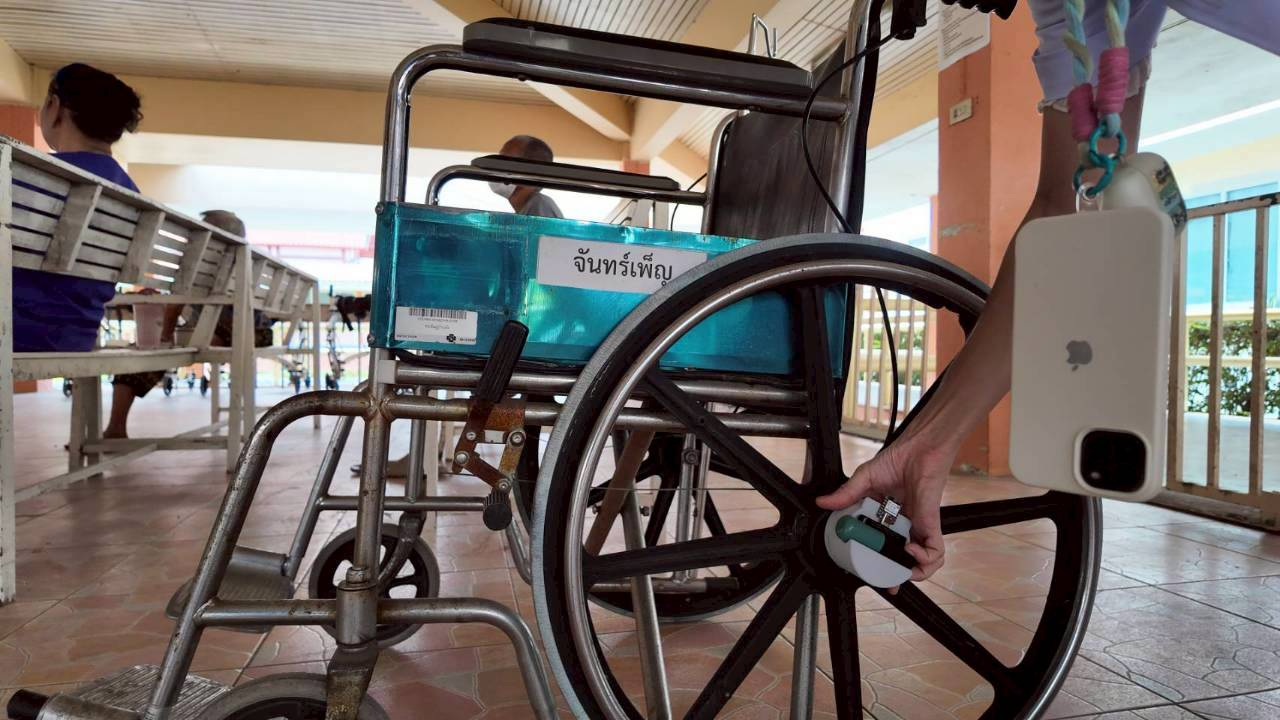
\includegraphics[width=\linewidth]{assets/appendices/legacy-field/wheelchair-install.jpg}
        \caption{การติดตั้งอุปกรณ์กับเก้าอี้รถเข็น}
        \label{fig:appI_wheelchair_install}
    \end{subfigure}
    \caption{ตัวอย่างการติดตั้งอุปกรณ์ในพื้นที่ทดสอบและบนเก้าอี้รถเข็น}
\end{figure}

\begin{figure}[!htbp]
    \centering
    \begin{subfigure}[t]{0.48\textwidth}
        \centering
        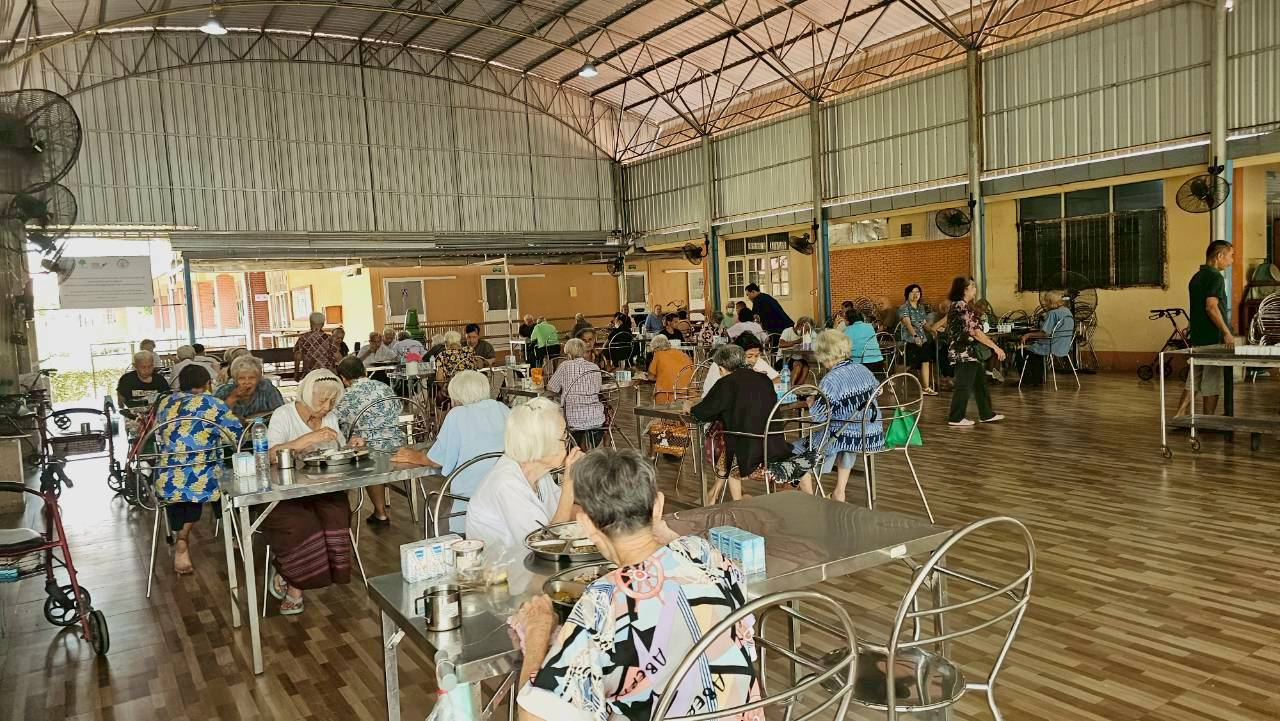
\includegraphics[width=\linewidth]{assets/appendices/legacy-field/elderly-home.jpg}
        \caption{บริบทผู้สูงอายุในสถานดูแล}
        \label{fig:appI_elderly_home}
    \end{subfigure}
    \hfill
    \begin{subfigure}[t]{0.48\textwidth}
        \centering
        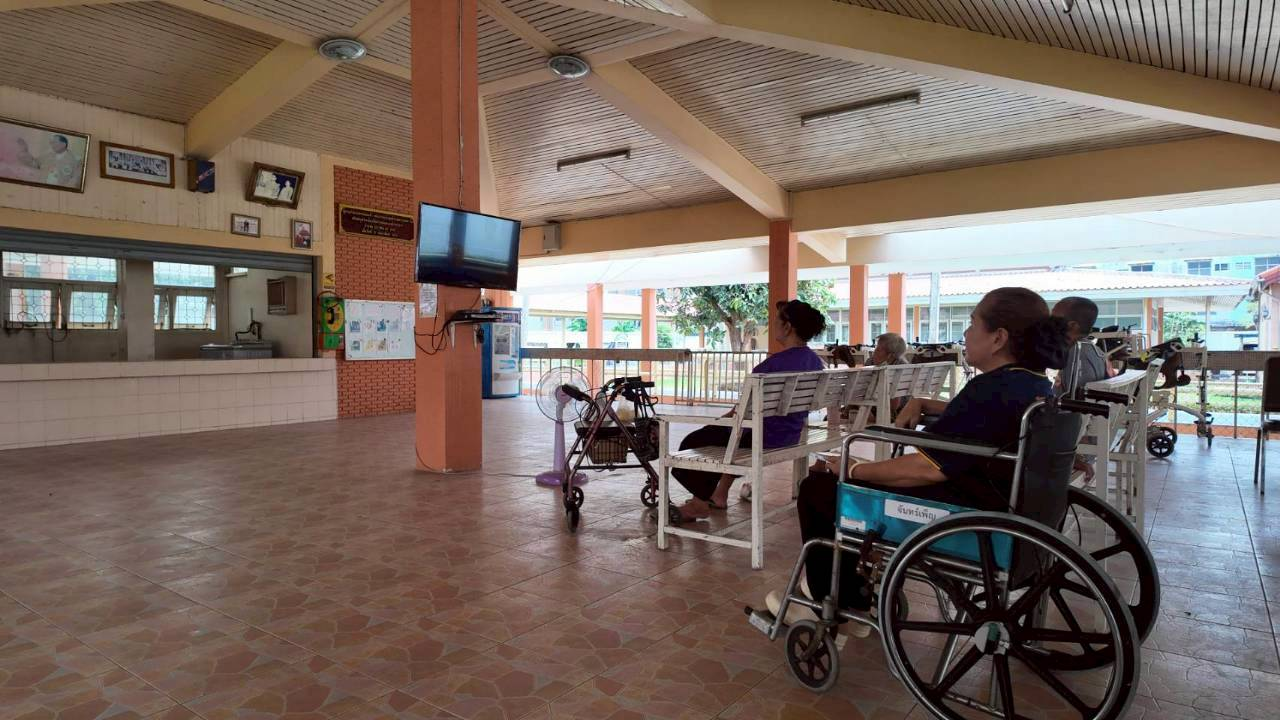
\includegraphics[width=\linewidth]{assets/appendices/legacy-field/elderly-device-use.jpg}
        \caption{การใช้งานอุปกรณ์ในบริบททดลอง}
        \label{fig:appI_elderly_device_use}
    \end{subfigure}
    \caption{บริบทผู้ใช้และการทดลองใช้อุปกรณ์ต้นแบบ}
\end{figure}

\begin{figure}[!htbp]
    \centering
    \begin{subfigure}[t]{0.48\textwidth}
        \centering
        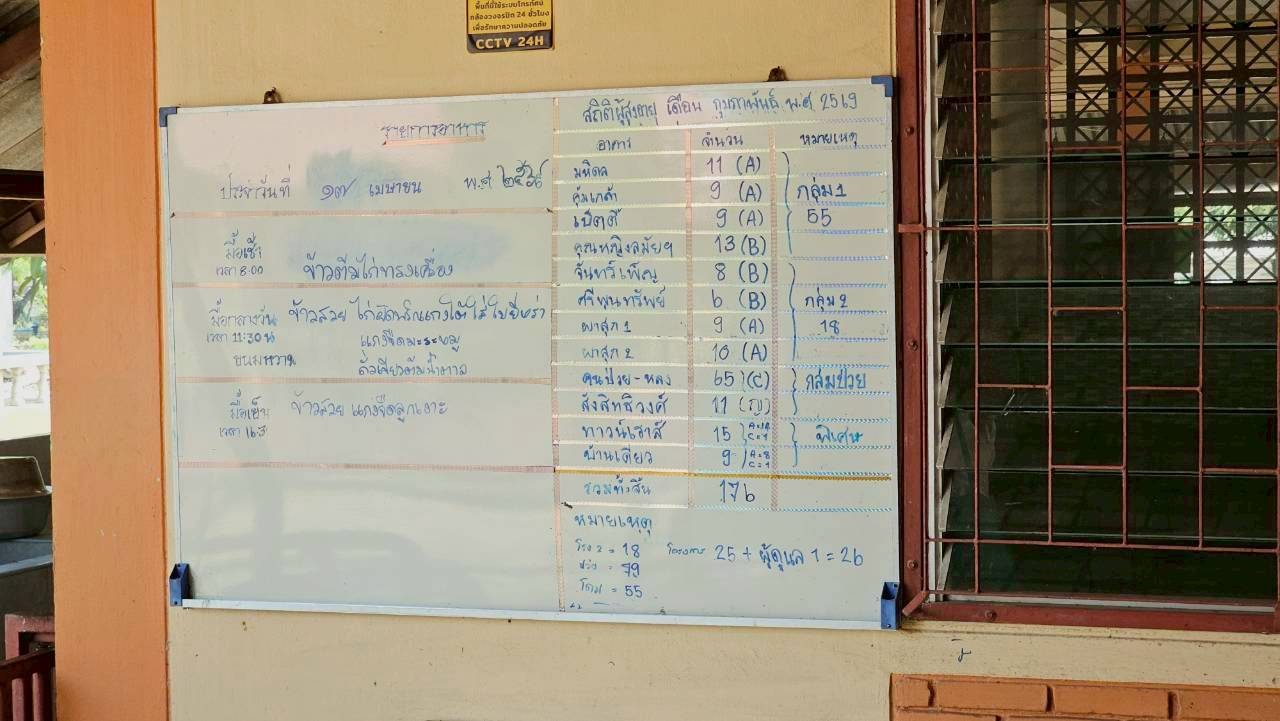
\includegraphics[width=\linewidth]{assets/appendices/legacy-field/workflow-board-1.jpg}
        \caption{บอร์ดแนวคิดการทำงานชุดที่ 1}
    \end{subfigure}
    \hfill
    \begin{subfigure}[t]{0.48\textwidth}
        \centering
        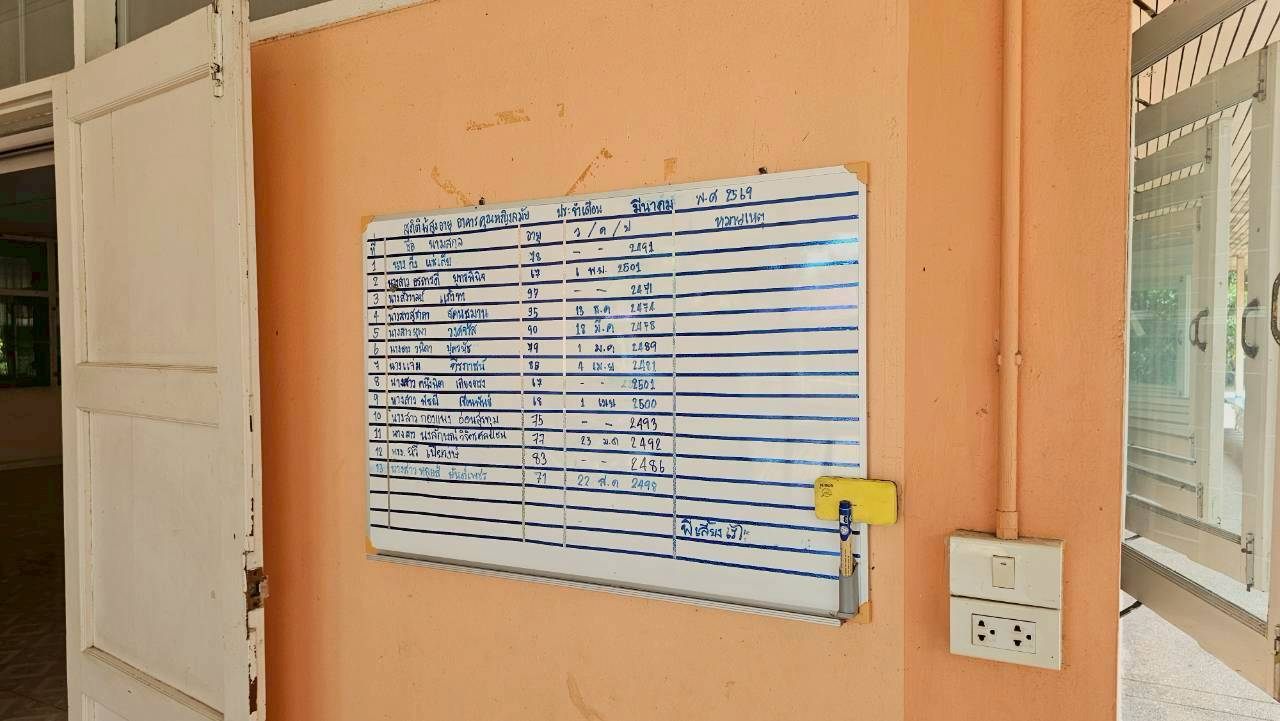
\includegraphics[width=\linewidth]{assets/appendices/legacy-field/workflow-board-2.jpg}
        \caption{บอร์ดแนวคิดการทำงานชุดที่ 2}
    \end{subfigure}
    \caption{ภาพประกอบการสรุปแนวคิดและ workflow ระหว่างการออกแบบระบบ}
    \label{fig:appI_workflow_boards}
\end{figure}

\begin{figure}[!htbp]
    \centering
    \begin{subfigure}[t]{0.48\textwidth}
        \centering
        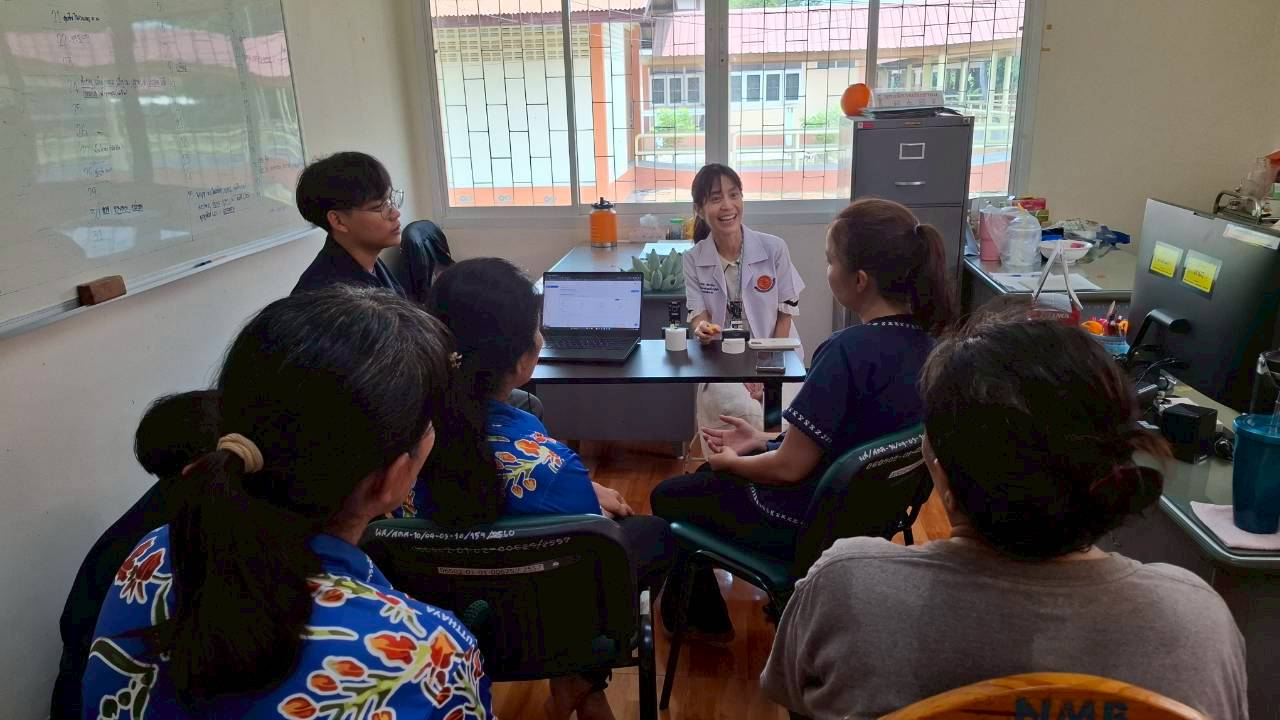
\includegraphics[width=\linewidth]{assets/appendices/legacy-field/caregiver-feedback.jpg}
        \caption{การอธิบายแนวทางใช้งานและรับฟังความคิดเห็น}
        \label{fig:appI_caregiver_feedback}
    \end{subfigure}
    \hfill
    \begin{subfigure}[t]{0.48\textwidth}
        \centering
        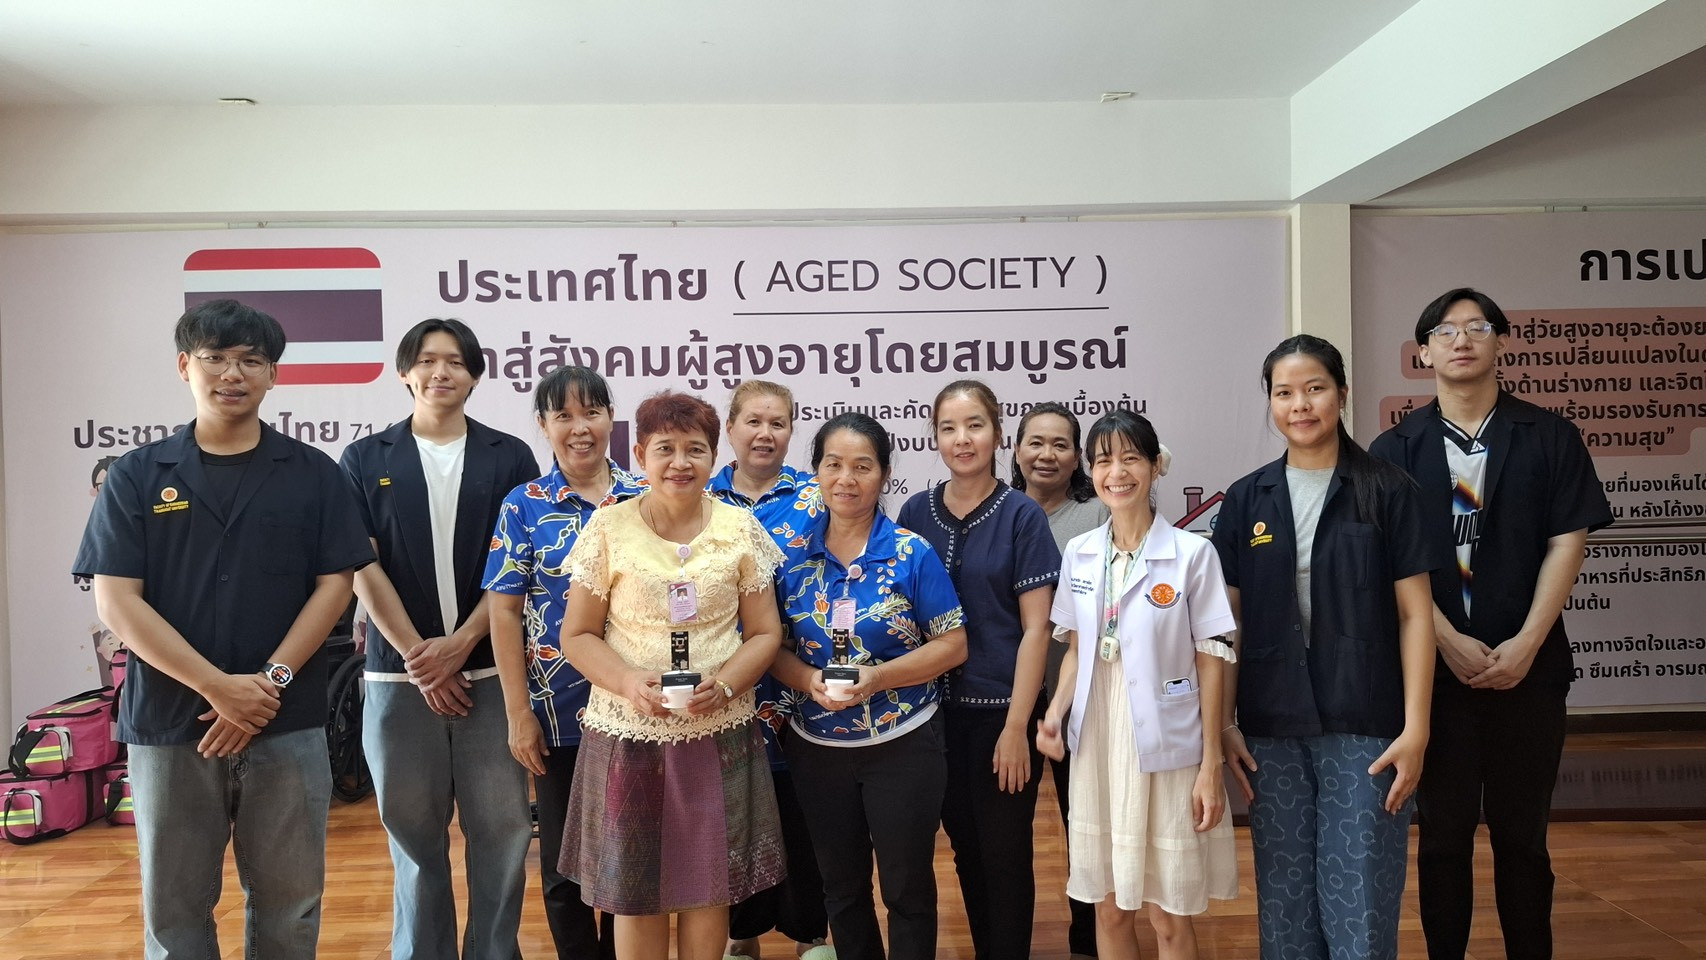
\includegraphics[width=\linewidth]{assets/appendices/legacy-field/group-photo.jpg}
        \caption{การลงพื้นที่และพูดคุยกับผู้เกี่ยวข้อง}
        \label{fig:appI_group_photo}
    \end{subfigure}
    \caption{ภาพประกอบการรับฟังความคิดเห็นและการลงพื้นที่}
\end{figure}
